\documentclass{article}
\usepackage[utf8]{inputenc}

\usepackage{graphicx}
\usepackage[2cm, right=2cm,top=2cm,bottom=2cm]{geometry}

\title{Microprocessor and Assembly Language Lab 04}
\author{Kazi Shadman Sakib, FH-97}
\date{March 04, 2022}

\begin{document}

\maketitle

\section{Task i} 

\subsection{Explaining two directives: Data and Align with proper example.}

\textbf{Data:} The data directive sets data as the current section. The lines that follow will be assembled into the data section. The data section is normally used to contain tables of data or pre-initialized variables.\newline\newline
\textbf{Example:}

AREA test\textunderscore data, DATA, READWRITE, ALIGN=2\newline
X DCB "Hello",0\newline
Y DCB "World",0\newline\newline
\textbf{Align:} The ALIGN directive aligns the current location to a specified boundary by padding with zeros or NOP instructions. Use ALIGN to ensure that your data and code is aligned to appropriate boundaries.\newline\newline
\textbf{Example:}

AREA test\textunderscore data, DATA, READWRITE, ALIGN=2\newline
X DCB "Hello",0\newline
Y DCB "World",0\newline\newline
The ALIGN directive tells the assembler that the next instruction is word aligned and offset by 2 bytes. DCB is followed by an instruction, use an ALIGN directive to ensure that the instruction is aligned.

\section{Task ii}

\subsection{Detailed Code Explanation}

The MRS instruction is used for copying the values of status register from APSR to general purpose register r0, from IPSR to general purpose register r1 and from EPSR to general purpose register r2. We update the flags by comparing value of 5 and 10 in register r3.

\subsection{Detailed Description of the Instruction Used to Design the Program.}

\item \textbf{MOV: }MOV copies the value specified in the second operand to the the specified register.
\item \textbf{CMP: }CMP compares the two operands (operand 1 and operand 2) and updates the status flags accordingly.
\item \textbf{MRS: }MRS copies the contents of a special purpose register to a general purpose register.

\subsection{Screenshot of Debugger}

\subsubsection{Status of the Status Registers After the Operation}

\begin{center}
    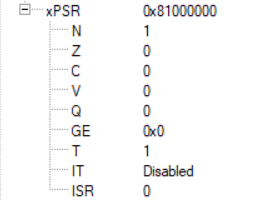
\includegraphics[width=0.5\textwidth]{task_ii_PSR.png}
\end{center}

\subsubsection{After the Code has been Loaded}

\begin{center}
    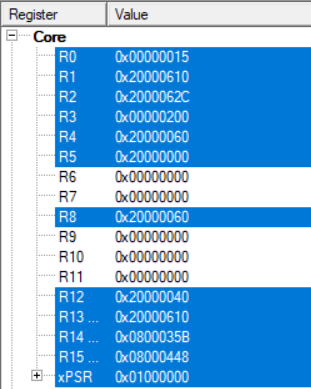
\includegraphics[width=0.5\textwidth]{task_ii_before.png}
\end{center}

\subsubsection{After the Code has been Executed}

\begin{center}
    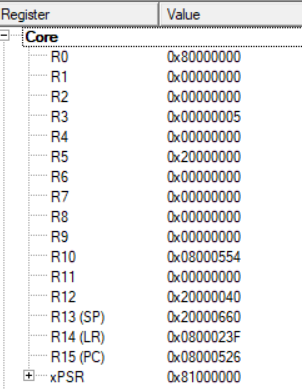
\includegraphics[width=0.5\textwidth]{task_ii_after.png}
\end{center}

\section{Task iii A}

\subsection{Detailed Code Explanation}
Firstly, We create an area for the variables, and allocate memory for the variables I and S. We load the contents of I and S to the register r1 and r2 respectively. Then we multiply the contents of register r1 with itself to get the square of I and add to the current sum. Then we increment I by 1. Then we check if the value of I is reached, and if not we loop again. When the loop has ended, we store the sum into the memory location of the variable S.

\subsection{Detailed Description of the Instruction Used to Design the Program.}

\item \textbf{DCD: }DCD allocates words of memory and defines the initial runtime contents of the memory.
\item \textbf{LDR: }LDR loads the words to the specified register.
\item \textbf{MUL: }:MUL multiplies the specified values and places the result in a register.
\item \textbf{ADD: }:ADD multiplies the specified values and places the result in a register.
\item \textbf{CMP: }CMP compares the two operands and updates the status flags.
\item \textbf{BLS: }BLS branches to specified label if the result of the compared value was lower or same than the other.
\item \textbf{STR: }STR stores the contents of the specified register to a memory location.

\subsection{Screenshot of Debugger}

\subsubsection{Status of the Status Registers After the Operation}

\begin{center}
    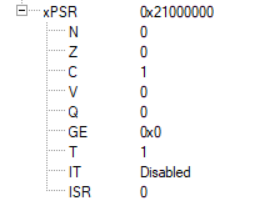
\includegraphics[width=0.5\textwidth]{task_iii_A_PSR.png}
\end{center}

\subsubsection{After the Code has been Loaded}

\begin{center}
    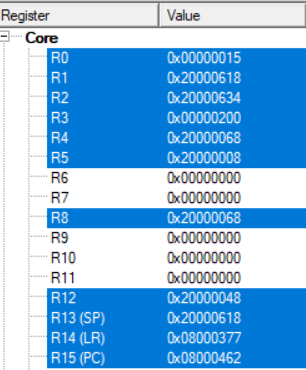
\includegraphics[width=0.5\textwidth]{task_iii_A_before.png}
\end{center}

\subsubsection{After the Code has been Executed}

\begin{center}
    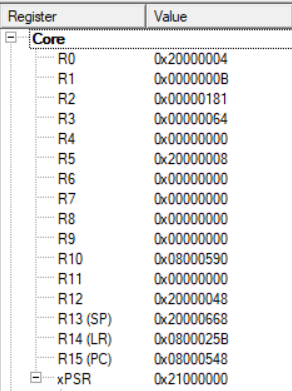
\includegraphics[width=0.5\textwidth]{task_iii_A_after.png}
\end{center}

\section{Task iii B}

\subsection{Detailed Code Explanation}
We create an area for the variables, and allocate memory for the variables and result. We load the contents of the variable A, B, C into the register r1, r2 and r3 respectively. Then we multiply the contents of each of r1, r2 and r3 to get the squares of the variables, and then we add the contents of r1 and r2 for the sum of their squares. We compare this value against the third square, and if they are equal, we set the value of r5 to 1 and store it to the memory location of the S variable.

\subsection{Detailed Description of the Instruction Used to Design the Program.}

\item \textbf{DCB: }DCB allocates bytes of memory and defines the initial runtime contents of the memory.
\item \textbf{LDR\{B\}: }LDR loads the words to the specified register. B stands for Byte.
\item \textbf{MUL: }:MUL multiplies the specified values and places the result in a register.
\item \textbf{ADD: }:ADD multiplies the specified values and places the result in a register.
\item \textbf{CMP: }CMP compares the two operands and updates the status flags.
\item \textbf{BEQ: }BEQ (short for "Branch if Equal") is the mnemonic for a machine language instruction which branches, or "jumps", to the address specified if, and only if the zero flag is set.
\item \textbf{STR: }STR stores the contents of the specified register to a memory location.

\subsection{Screenshot of Debugger}

\subsubsection{Status of the Status Registers After the Operation}

\begin{center}
    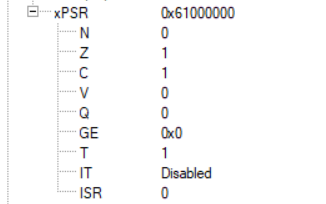
\includegraphics[width=0.5\textwidth]{task_iii_B_PSR.png}
\end{center}

\subsubsection{After the Code has been Loaded}

\begin{center}
    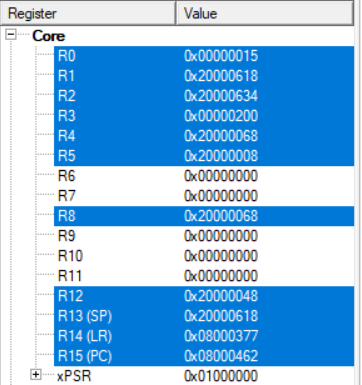
\includegraphics[width=0.5\textwidth]{task_iii_B_before.png}
\end{center}

\subsubsection{After the Code has been Executed}

\begin{center}
    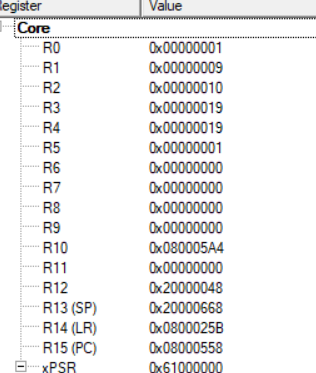
\includegraphics[width=0.5\textwidth]{task_iii_B_after.png}
\end{center}

\section{Task iv A}

\subsection{Detailed Code Explanation}
We create an area for the variables, and allocate memory for the strings. We load the address of the first byte of strings X and Y to the registers r0 and r1 respectively. Then we load the current byte of the string X to r2 and increment the stored address to point to the next byte. Then we store the byte loaded to r2, into the address of Y and increment it. We check if the end of the string is reached, and if not then we loop. Otherwise we copy the entire string and end execution.

\subsection{Detailed Description of the Instruction Used to Design the Program.}

\item \textbf{DCB: }DCB allocates bytes of memory and defines the initial runtime contents of the memory.
\item \textbf{LDR\{B\}: }LDR loads the words to the specified register. B stands for Byte.
\item \textbf{CMP: }CMP compares the two operands and updates the status flags.
\item \textbf{BNE: }BNE branches to specified label if the result of the compared values were not equal.
\item \textbf{STR\{B\}: }STR stores the contents of the specified register to a memory location. B stands for Byte.

\subsection{Screenshot of Debugger}

\subsubsection{Status of the Status Registers After the Operation}

\begin{center}
    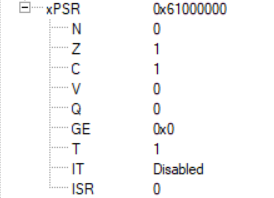
\includegraphics[width=0.5\textwidth]{task_iv_A_PSR.png}
\end{center}

\subsubsection{After the Code has been Loaded}

\begin{center}
    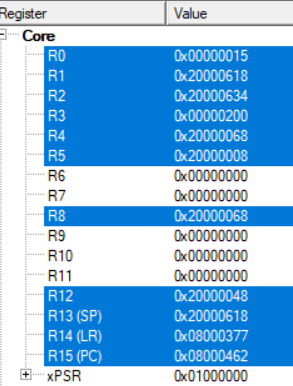
\includegraphics[width=0.5\textwidth]{task_iv_A_before.png}
\end{center}

\subsubsection{After the Code has been Executed}

\begin{center}
    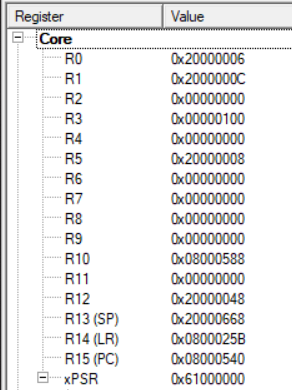
\includegraphics[width=0.5\textwidth]{task_iv_A_after.png}
\end{center}

\section{Task iv B}

\subsection{Detailed Code Explanation}
We create an area for the variables, and allocate memory for the strings. We load the address of the first bytes strings X and Y to the registers r1 and r2 respectively. We also load the immediate address before the string X in the register r0. Then we load the current or first byte of the string X to r3 and increment the stored address to point to the next byte. We check if the end of the string is reached, and if not then we loop. Otherwise we reach the end of the string and have that address in the register r1. Then we start loading bytes from the last address of the string X in r1 and decrement it until we reach the start of the string, and store the bytes in reverse order in the memory location of Y.

\subsection{Detailed Description of the Instruction Used to Design the Program.}

\item \textbf{DCB: }DCB allocates bytes of memory and defines the initial runtime contents of the memory.
\item \textbf{LDR\{B\}: }LDR loads the words to the specified register. B stands for Byte.
\item \textbf{ADD: }:ADD multiplies the specified values and places the result in a register.
\item \textbf{CMP: }CMP compares the two operands and updates the status flags.
\item \textbf{BNE: }BNE branches to specified label if the result of the compared values were not equal.
\item \textbf{STR\{B\}: }STR stores the contents of the specified register to a memory location. B stands for Byte.

\subsection{Screenshot of Debugger}

\subsubsection{Status of the Status Registers After the Operation}

\begin{center}
    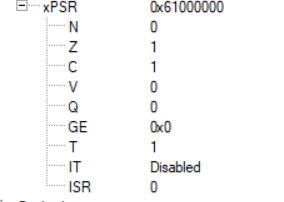
\includegraphics[width=0.5\textwidth]{task_iv_B_PSR.png}
\end{center}

\subsubsection{After the Code has been Loaded}

\begin{center}
    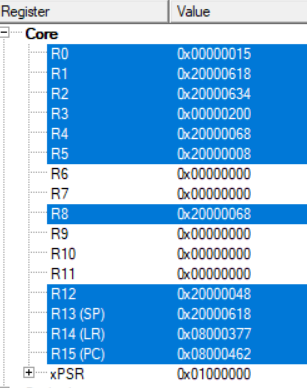
\includegraphics[width=0.5\textwidth]{task_iv_B_before.png}
\end{center}

\subsubsection{After the Code has been Executed}

\begin{center}
    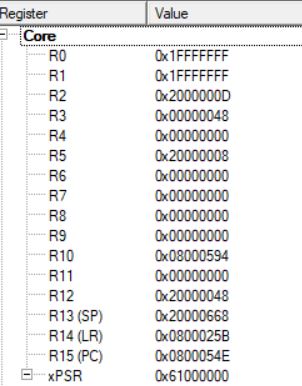
\includegraphics[width=0.5\textwidth]{task_iv_B_after.png}
\end{center}

\section{Task iv C}

\subsection{Detailed Code Explanation}
We create an area for the variables, and allocate memory for the strings. We load the address of the first bytes of the string X to the register r0. Then we load the current or first byte of the string X to r1 and increment the stored address to point to the next byte. Then we increment the value of r2, which we initialized to 0. We check if the end of the string is reached, and if not then we loop. Otherwise we find the length the entire string and decrement by 1 to remove null character and end execution.

\subsection{Detailed Description of the Instruction Used to Design the Program.}

\item \textbf{DCB: }DCB allocates bytes of memory and defines the initial runtime contents of the memory.
\item \textbf{LDR\{B\}: }LDR loads the words to the specified register. B stands for Byte.
\item \textbf{MOV: }MOV copies the value specified in the second operand to the the specified register.
\item \textbf{ADD: }:ADD multiplies the specified values and places the result in a register.
\item \textbf{CMP: }CMP compares the two operands and updates the status flags.
\item \textbf{BNE: }BNE branches to specified label if the result of the compared values were not equal.

\subsection{Screenshot of Debugger}

\subsubsection{Status of the Status Registers After the Operation}

\begin{center}
    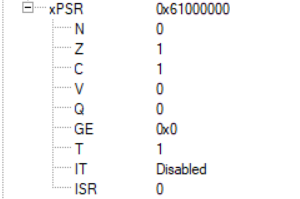
\includegraphics[width=0.5\textwidth]{task_iv_C_PSR.png}
\end{center}

\subsubsection{After the Code has been Loaded}

\begin{center}
    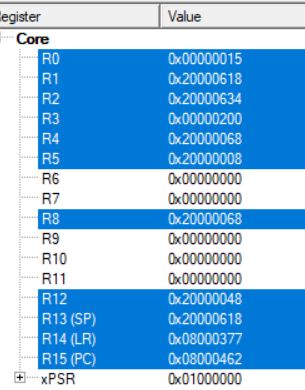
\includegraphics[width=0.5\textwidth]{task_iv_C_before.png}
\end{center}

\subsubsection{After the Code has been Executed}

\begin{center}
    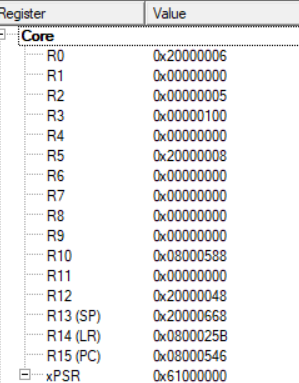
\includegraphics[width=0.5\textwidth]{task_iv_C_after.png}
\end{center}

\section{Task iv D}

\subsection{Detailed Code Explanation}
We create an area for the variables, and allocate memory for the strings. We load the address of the first bytes strings X and Y to the registers r0 and r1 respectively. Then we load the current byte of X and Y to the registers r2 and r3, and check if any of them have reached the end of the string, and if so, go to exit. Otherwise we compare the values of the two characters, and if they are the same we loop again, otherwise we exit the loop. After exiting, we compare the last two characters, if the loop exited with both being equal, then this last compare would reflect it and update flags accordingly.

\subsection{Detailed Description of the Instruction Used to Design the Program.}

\item \textbf{DCB: }DCB allocates words of memory and defines the initial runtime contents of the memory.
\item \textbf{LDR\{B\}: }LDR loads the words to the specified register. B stands for Byte.
\item \textbf{CMP: }CMP compares the two operands and updates the status flags.
\item \textbf{BEQ: }BEQ branches to specified label if the result of the compared values were equal.
\item \textbf{BNB: }BNE branches to specified label if the result of the compared values were not equal.

\subsection{Screenshot of Debugger}

\subsubsection{Status of the Status Registers After the Operation}

\begin{center}
    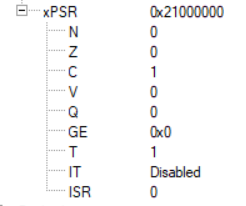
\includegraphics[width=0.5\textwidth]{task_iv_D_PSR.png}
\end{center}

\subsubsection{After the Code has been Loaded}

\begin{center}
    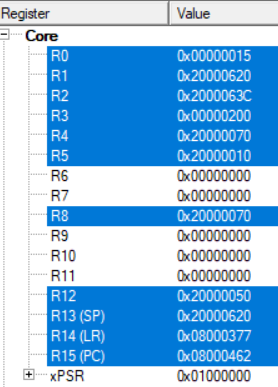
\includegraphics[width=0.5\textwidth]{task_iv_D_before.png}
\end{center}

\subsubsection{After the Code has been Executed}

\begin{center}
    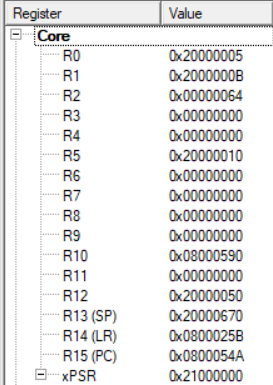
\includegraphics[width=0.5\textwidth]{task_iv_D_after.png}
\end{center}

\section{Task iv E}

\subsection{Detailed Code Explanation}
 We create an area for the variables, and allocate memory for the strings. We load the address of the first bytes strings X and Y to the registers r0 and r1 respectively. Then we load the current or first byte of the string X to r2 and increment the stored address to point to the next byte. We check if the end of the string is reached, and if not then we loop. Otherwise we reach the end of the string and that address is stored in the register r0. Then we load the current or first byte of the string Y to r2 and increment that by 1, and store that byte to the address stored in r0. Then we check if the end of the string Y is reached, otherwise we loop. As a result, the two strings will be concatenated. We create an area for the variables, and allocate memory for the strings.

\subsection{Detailed Description of the Instruction Used to Design the Program.}

\item \textbf{DCB: }DCB allocates bytes of memory and defines the initial runtime contents of the memory.
\item \textbf{LDR\{B\}: }LDR loads the words to the specified register. B stands for Byte.
\item \textbf{CMP: }CMP compares the two operands and updates the status flags.
\item \textbf{BNE: }BNE branches to specified label if the result of the compared values were not equal.
\item \textbf{STR\{B\}: }STR stores the contents of the specified register to a memory location. B stands for Byte.

\subsection{Screenshot of Debugger}

\subsubsection{Status of the Status Registers After the Operation}

\begin{center}
    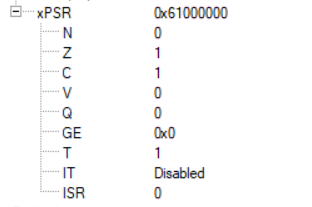
\includegraphics[width=0.5\textwidth]{task_iv_E_PSR.png}
\end{center}

\subsubsection{After the Code has been Loaded}

\begin{center}
    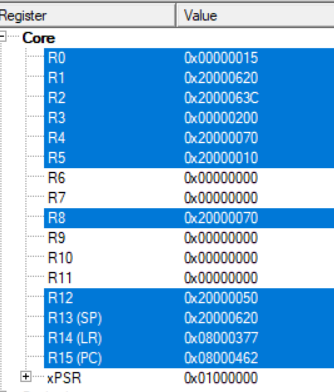
\includegraphics[width=0.5\textwidth]{task_iv_E_before.png}
\end{center}

\subsubsection{After the Code has been Executed}

\begin{center}
    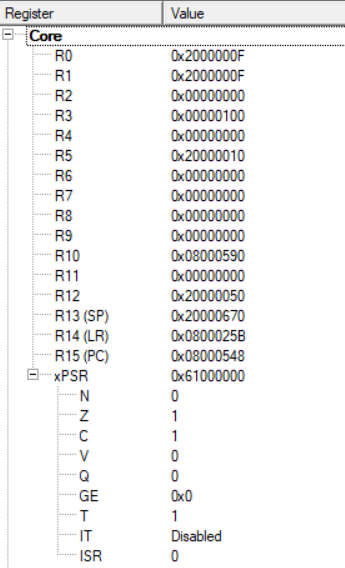
\includegraphics[width=0.5\textwidth]{task_iv_E_after.png}
\end{center}

\end{document}
